Рассмотрим систему массового обслуживания $M|H_{2}|N$ с обратной связью (Рисунок \ref{fig:systemN}).

\begin{figure}[htbp]
	\centering
	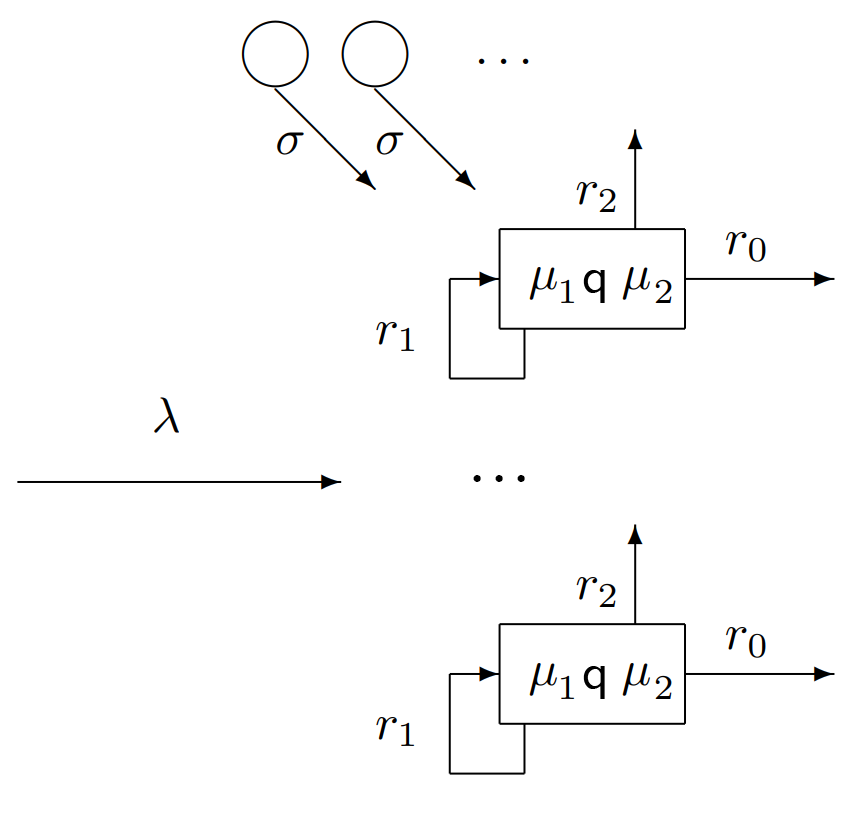
\includegraphics[width=0.5\textwidth]{systemN}
	\caption{Система массового обслуживания $M|H_{2}|N$ с обратной связью}
	\label{fig:systemN}
\end{figure}


Система имеет $N$ обслуживающих приборов. Заявки поступают в систему согласно простейщиму потоку с параметром $\lambda$. Каждая заявка занимеет один из свободных приборов на время, распределенное по гиперэкспоненциальному закону. Это означает, что заявка на приборе с вероятностью $q$ поступает на первую фазу, с экспоненциальным распределением с параметром $\mu_{1}$, и с вероятность $1-q$ на вторую, с параметром $\mu_{2}$.

После завершения обслуживания заявка с вероятностью $r_{0}$ покидает систему, с вероятностью $r_{1}$ мгновенно поступает на повторное обслуживание и с вероятностью $r_{2}$ уходит на орбиту. Также, если на момент поступления заявки из потока все приборы заняты, то заявка уходит на орбиту. Через время, продолжительность которого распределена по экспоненциальному закону с пареметром $\sigma$, заявка вновь обращается с орбиты к приборам.

Пусть $i(t)$ -- число заявок на орбите в момент времени $t$, 
$n_{1}(t)$ -- число приборов занятых на первой фазе в момент времени $t$,
$n_{2}(t)$ -- число приборов занятых на второй фазе в момент времени $t$.

Рассмотрим трехмерный процесс $\{n_{1}(t), n_{2}(t), i(t)\}$. Под состоянием системы будем понимать состояние процесса $\{n_{1}(t), n_{2}(t), i(t)\}$ в момент времени $t$.

 Обозначим вероятности следующим образом \\
 \begin{center}
 	$P(n_{1}(t) = n_{2}, n_{2}(t)=n_{2}, i(t)=i)$= $P_{n_{1},n_{2}}$(i,t)\\
 \end{center}
вероятность того, что $n_{1}$ -- приборов занято на первой фазе, а $n_{2}$ -- приборов занято на второй фазе. При этом  $P_{n_{1},n_{2}}(i,t)=0$, если $n_{1}$ < 0, $n_{2}$ < 0 или $n_{1}+n_{2} > N.$\\

Для решения будем применять методы асимптотически анализа предложенные в [ 5, 8, 12, 21] и асимптотически диффузионного анализа предложенные в [21].

